
\documentclass[a4paper,11pt]{article}
\usepackage[a4paper, margin=8em]{geometry}

% usa i pacchetti per la scrittura in italiano
\usepackage[french,italian]{babel}
\usepackage[T1]{fontenc}
\usepackage[utf8]{inputenc}
\frenchspacing 

% usa i pacchetti per la formattazione matematica
\usepackage{amsmath, amssymb, amsthm, amsfonts}

% usa altri pacchetti
\usepackage{gensymb}
\usepackage{hyperref}
\usepackage{standalone}

\usepackage{colortbl}

\usepackage{xstring}
\usepackage{karnaugh-map}

% imposta il titolo
\title{Electronics for Embedded Systems notes}
\author{Luca Seggiani}
\date{2026}

% spaziatura liste
\usepackage{enumitem}
\setlist[itemize]{noitemsep, topsep=4pt, partopsep=0pt, parsep=2pt, leftmargin=*}
\setlist[enumerate]{noitemsep, topsep=4pt, partopsep=0pt, parsep=2pt, leftmargin=*}

% imposta lo stile
% usa helvetica
\usepackage[scaled]{helvet}
% usa palatino
\usepackage{palatino}
% usa un font monospazio guardabile
\usepackage{lmodern}

\renewcommand{\rmdefault}{ppl}
\renewcommand{\sfdefault}{phv}
\renewcommand{\ttdefault}{lmtt}

% circuiti
\usepackage{circuitikz}
\usetikzlibrary{babel}

% testo cerchiato
\newcommand*\circled[1]{\tikz[baseline=(char.base)]{
            \node[shape=circle,draw,inner sep=2pt] (char) {#1};}}

% disponi il titolo
\makeatletter
\renewcommand{\maketitle} {
	\begin{center} 
		\begin{minipage}[t]{.8\textwidth}
			\textsf{\huge\bfseries \@title} 
		\end{minipage}%
		\begin{minipage}[t]{.2\textwidth}
			\raggedleft \vspace{-1.65em}
			\textsf{\small \@author} \vfill
			\textsf{\small \@date}
		\end{minipage}
		\par
	\end{center}

	\thispagestyle{empty}
	\pagestyle{fancy}
}
\makeatother

% disponi teoremi
\usepackage{tcolorbox}
\newtcolorbox[auto counter, number within=section]{theorem}[2][]{%
	colback=blue!10, 
	colframe=blue!40!black, 
	sharp corners=northwest,
	fonttitle=\sffamily\bfseries, 
	title=Theorem~\thetcbcounter: #2, 
	#1
}

% disponi definizioni
\newtcolorbox[auto counter, number within=section]{definition}[2][]{%
	colback=red!10,
	colframe=red!40!black,
	sharp corners=northwest,
	fonttitle=\sffamily\bfseries,
	title=Definition~\thetcbcounter: #2,
	#1
}

% disponi codice
\usepackage{listings}
\usepackage[table]{xcolor}

\definecolor{codegreen}{rgb}{0,0.6,0}
\definecolor{codegray}{rgb}{0.5,0.5,0.5}
\definecolor{codepurple}{rgb}{0.58,0,0.82}
\definecolor{backcolour}{rgb}{0.95,0.95,0.92}

\lstdefinestyle{codestyle}{
		backgroundcolor=\color{black!5}, 
		commentstyle=\color{codegreen},
		keywordstyle=\bfseries\color{magenta},
		numberstyle=\sffamily\tiny\color{black!60},
		stringstyle=\color{green!50!black},
		basicstyle=\ttfamily\footnotesize,
		breakatwhitespace=false,         
		breaklines=true,                 
		captionpos=b,                    
		keepspaces=true,                 
		numbers=left,                    
		numbersep=5pt,                  
		showspaces=false,                
		showstringspaces=false,
		showtabs=false,                  
		tabsize=2
}

\lstdefinestyle{shellstyle}{
		backgroundcolor=\color{black!5}, 
		basicstyle=\ttfamily\footnotesize\color{black}, 
		commentstyle=\color{black}, 
		keywordstyle=\color{black},
		numberstyle=\color{black!5},
		stringstyle=\color{black}, 
		showspaces=false,
		showstringspaces=false, 
		showtabs=false, 
		tabsize=2, 
		numbers=none, 
		breaklines=true
}

\lstdefinelanguage{x86}{ 
  keywords={AAA, AAD, AAM, AAS, ADC, ADCB, ADCW, ADCL, ADD, ADDB, ADDW, ADDL, AND, ANDB, ANDW, ANDL,
        ARPL, BOUND, BSF, BSFL, BSFW, BSR, BSRL, BSRW, BSWAP, BT, BTC, BTCB, BTCW, BTCL, BTR, 
        BTRB, BTRW, BTRL, BTS, BTSB, BTSW, BTSL, CALL, CBW, CDQ, CLC, CLD, CLI, CLTS, CMC, CMP,
        CMPB, CMPW, CMPL, CMPS, CMPSB, CMPSD, CMPSW, CMPXCHG, CMPXCHGB, CMPXCHGW, CMPXCHGL,
        CMPXCHG8B, CPUID, CWDE, DAA, DAS, DEC, DECB, DECW, DECL, DIV, DIVB, DIVW, DIVL, ENTER,
        HLT, IDIV, IDIVB, IDIVW, IDIVL, IMUL, IMULB, IMULW, IMULL, IN, INB, INW, INL, INC, INCB,
        INCW, INCL, INS, INSB, INSD, INSW, INT, INT3, INTO, INVD, INVLPG, IRET, IRETD, JA, JAE,
        JB, JBE, JC, JCXZ, JE, JECXZ, JG, JGE, JL, JLE, JMP, JNA, JNAE, JNB, JNBE, JNC, JNE, JNG,
        JNGE, JNL, JNLE, JNO, JNP, JNS, JNZ, JO, JP, JPE, JPO, JS, JZ, LAHF, LAR, LCALL, LDS,
        LEA, LEAVE, LES, LFS, LGDT, LGS, LIDT, LMSW, LOCK, LODSB, LODSD, LODSW, LOOP, LOOPE,
        LOOPNE, LSL, LSS, LTR, MOV, MOVB, MOVW, MOVL, MOVSB, MOVSD, MOVSW, MOVSX, MOVSXB,
        MOVSXW, MOVSXL, MOVZX, MOVZXB, MOVZXW, MOVZXL, MUL, MULB, MULW, MULL, NEG, NEGB, NEGW,
        NEGL, NOP, NOT, NOTB, NOTW, NOTL, OR, ORB, ORW, ORL, OUT, OUTB, OUTW, OUTL, OUTSB, OUTSD,
        OUTSW, POP, POPL, POPW, POPB, POPA, POPAD, POPF, POPFD, PUSH, PUSHL, PUSHW, PUSHB, PUSHA, 
        RCLL, RCR, RCRB, RCRW, RCRL, RDMSR, RDPMC, RDTSC, REP, REPE, REPNE, RET, ROL, ROLB, ROLW,
        ROLL, ROR, RORB, RORW, RORL, SAHF, SAL, SALB, SALW, SALL, SAR, SARB, SARW, SARL, SBB,
        SBBB, SBBW, SBBL, SCASB, SCASD, SCASW, SETA, SETAE, SETB, SETBE, SETC, SETE, SETG, SETGE,
        SETL, SETLE, SETNA, SETNAE, SETNB, SETNBE, SETNC, SETNE, SETNG, SETNGE, SETNL, SETNLE,
        SETNO, SETNP, SETNS, SETNZ, SETO, SETP, SETPE, SETPO, SETS, SETZ, SGDT, SHL, SHLB, SHLW,
        SHLL, SHLD, SHR, SHRB, SHRW, SHRL, SHRD, SIDT, SLDT, SMSW, STC, STD, STI, STOSB, STOSD,
        STOSW, STR, SUB, SUBB, SUBW, SUBL, TEST, TESTB, TESTW, TESTL, VERR, VERW, WAIT, WBINVD,
        XADD, XADDB, XADDW, XADDL, XCHG, XCHGB, XCHGW, XCHGL, XLAT, XLATB, XOR, XORB, XORW, XORL},
  keywordstyle=\color{blue}\bfseries,
  ndkeywordstyle=\color{darkgray}\bfseries,
  identifierstyle=\color{black},
  sensitive=false,
  comment=[l]{\#},
  morecomment=[s]{/*}{*/},
  commentstyle=\color{purple}\ttfamily,
  stringstyle=\color{red}\ttfamily,
  morestring=[b]',
  morestring=[b]"
}

\lstdefinelanguage{riscv}{
  keywords={
    LUI, AUIPC,
    JAL, JALR,
    BEQ, BNE, BLT, BGE, BLTU, BGEU,
    LB, LH, LW, LBU, LHU, LD,
    SB, SH, SW, SD,
    ADDI, SLTI, SLTIU, XORI, ORI, ANDI,
    SLLI, SRLI, SRAI,
    ADD, SUB, SLL, SLT, SLTU, XOR, SRL, SRA, OR, AND,
    ADDIW, SLLIW, SRLIW, SRAIW,
    ADDW, SUBW, SLLW, SRLW, SRAW,
    MUL, MULH, MULHSU, MULHU, DIV, DIVU, REM, REMU,
    MULW, DIVW, DIVUW, REMW, REMUW,
    LR.W, SC.W, AMOSWAP.W, AMOADD.W, AMOXOR.W,
    AMOAND.W, AMOOR.W, AMOMIN.W, AMOMAX.W,
    AMOMINU.W, AMOMAXU.W,
    LR.D, SC.D, AMOSWAP.D, AMOADD.D, AMOXOR.D,
    AMOAND.D, AMOOR.D, AMOMIN.D, AMOMAX.D,
    AMOMINU.D, AMOMAXU.D,
    FLW, FSW,
    FMADD.S, FMSUB.S, FNMSUB.S, FNMADD.S,
    FADD.S, FSUB.S, FMUL.S, FDIV.S, FSQRT.S,
    FSGNJ.S, FSGNJN.S, FSGNJX.S,
    FMIN.S, FMAX.S,
    FCVT.W.S, FCVT.WU.S, FCVT.S.W, FCVT.S.WU,
    FMV.X.W, FMV.W.X,
    FEQ.S, FLT.S, FLE.S,
    FLD, FSD,
    FMADD.D, FMSUB.D, FNMSUB.D, FNMADD.D,
    FADD.D, FSUB.D, FMUL.D, FDIV.D, FSQRT.D,
    FSGNJ.D, FSGNJN.D, FSGNJX.D,
    FMIN.D, FMAX.D,
    FCVT.W.D, FCVT.WU.D, FCVT.D.W, FCVT.D.WU,
    FCVT.S.D, FCVT.D.S,
    FMV.X.D, FMV.D.X,
    FEQ.D, FLT.D, FLE.D,
    CSRRW, CSRRS, CSRRC,
    CSRRWI, CSRRSI, CSRRCI,
    FENCE.I,
    FENCE,
    ECALL, EBREAK,
    MRET, SRET, URET,
    WFI,
    SFENCE.VMA,
    NOP, LI, LA, MV,
    NOT, NEG, NEGW,
    SEQZ, SNEZ, SLTZ, SGTZ,
    BEQZ, BNEZ, BLEZ, BGEZ, BLTZ, BGTZ,
    BGT, BLE, BGTU, BLEU,
    J, JR, RET,
    CALL, TAIL,
    RDINSTRET, RDCYCLE, RDTIME,
    CSRR, CSRW, CSRS, CSRC,
    CSRWI, CSRSI, CSRCI
  },
  keywordstyle=\color{blue}\bfseries,
  ndkeywordstyle=\color{darkgray}\bfseries,
  identifierstyle=\color{black},
  sensitive=false,
  comment=[l]{\#},
  morecomment=[s]{/*}{*/},
  commentstyle=\color{purple}\ttfamily,
  stringstyle=\color{red}\ttfamily,
  morestring=[b]',
  morestring=[b]"
}

\lstdefinelanguage{arm}{
  keywords={
    ADC, ADD, AND, BIC, CMN, CMP, EOR, MOV, MVN,
    RSB, RSC, SBC, SUB, TST, TEQ,
    MLA, MLS, MUL, SMLAL, SMULL, UMLAL, UMULL,
    QADD, QSUB, QDADD, QDSUB,
    QADD16, QADD8, QASX, QSAX,
    QSUB16, QSUB8, QSAX, QSUBADDX,
    ASR, LSL, LSR, ROR, RRX,
    B, BL, BX, BLX,
    BXJ,
    BEQ, BNE, BCS, BHS, BCC, BLO,
    BMI, BPL, BVS, BVC,
    BHI, BLS, BGE, BLT, BGT, BLE,
    BAL,
    LDR, LDRB, LDRH, LDRSB, LDRSH,
    LDRD, LDM, LDMIA, LDMIB, LDMDA, LDMDB,
    LDRT, LDRBT, LDRHT, LDRSBT, LDRSHT,
    STR, STRB, STRH, STRD,
    STM, STMIA, STMIB, STMDA, STMDB,
    STRT, STRBT, STRHT,
    PUSH, POP,
    SWP, SWPB,
    REV, REV16, REVSH,
    BFC, BFI, BFXIL, SBFX, UBFX,
    CLZ,
    LDREX, LDREXB, LDREXH, LDREXD,
    STREX, STREXB, STREXH, STREXD,
    DMB, DSB, ISB,
    MCR, MCRR, MRC, MRRC,
    MRS, MSR,
    CPS, SETEND, SVC, BKPT,
    CLREX, WFE, WFI, SEV,
    YIELD, NOP,
    VLDR, VSTR,
    VMOV, VABS, VNEG,
    VADD, VSUB, VMUL, VDIV,
    VMLA, VMLS, VNMLA, VNMLS, VNMUL,
    VMAX, VMIN,
    VSQRT,
    VCMP, VCMPE,
    VCVT,
    VCLZ, VCLS,
    VAND, VORR, VEOR, VBIC, VMVN,
    VLD1, VLD2, VLD3, VLD4,
    VST1, VST2, VST3, VST4,
    ADR, ADCS, ADDS, SUBS, MOVS, ANDS, ORRS, EORS
  },
  keywordstyle=\color{blue}\bfseries,
  ndkeywordstyle=\color{darkgray}\bfseries,
  identifierstyle=\color{black},
  sensitive=false,
  comment=[l]{@},
  morecomment=[l]{;},
  morecomment=[s]{/*}{*/},
  commentstyle=\color{purple}\ttfamily,
  stringstyle=\color{red}\ttfamily,
  morestring=[b]',
  morestring=[b]"
}

\lstset{style=codestyle, language=C}

% disponi sezioni
\usepackage{titlesec}

\titleformat{\section}
	{\sffamily\Large\bfseries} 
	{\thesection}{1em}{} 
\titleformat{\subsection}
	{\sffamily\large\bfseries}   
	{\thesubsection}{1em}{} 
\titleformat{\subsubsection}
	{\sffamily\normalsize\bfseries} 
	{\thesubsubsection}{1em}{}

% tikz
\usepackage{tikz}

% float
\usepackage{float}

% grafici
\usepackage{pgfplots}
\pgfplotsset{width=10cm,compat=1.9}

% disponi alberi
\usepackage{forest}

\forestset{
	rectstyle/.style={
		for tree={rectangle,draw,font=\large\sffamily}
	},
	roundstyle/.style={
		for tree={circle,draw,font=\large}
	}
}

% disponi algoritmi
\usepackage{algorithm}
\usepackage{algorithmic}
\makeatletter
\renewcommand{\ALG@name}{Algorithm}
\makeatother

% disponi numeri di pagina
\usepackage{fancyhdr}
\fancyhf{} 
\fancyfoot[L]{\sffamily{\thepage}}

\makeatletter
\fancyhead[L]{\raisebox{1ex}[0pt][0pt]{\sffamily{\@title \ \@date}}} 
\fancyhead[R]{\raisebox{1ex}[0pt][0pt]{\sffamily{\@author}}}
\makeatother

\begin{document}
% sezione (data)
\section{Lesson 21-10-26}

% stili pagina
\thispagestyle{empty}
\pagestyle{fancy}

% testo
\subsubsection{FPGA LUTs}

Let's look at FPGA \textit{Look-Up Tables} (\textbf{LUT}s) in detail.
A LUT basically implements an $n$-input, $1$-output combinational logic circuit, made up of:
\begin{itemize}
	\item $2^n$ SRAM bit cells;
	\item A $2^n \rightarrow 1$ multiplexer, with $n$ selection inputs.
\end{itemize}

Note that an $n$-input,-$1$-output LUT is like a $2^n \times 1$ memory with:
\begin{itemize}
\item A single row, so need of a row decoder, and a row that is always selected;
\item $2^n$ columns, where the MUX is the column decoder and column multiplexer of the memory.
\end{itemize}

\begin{center}
	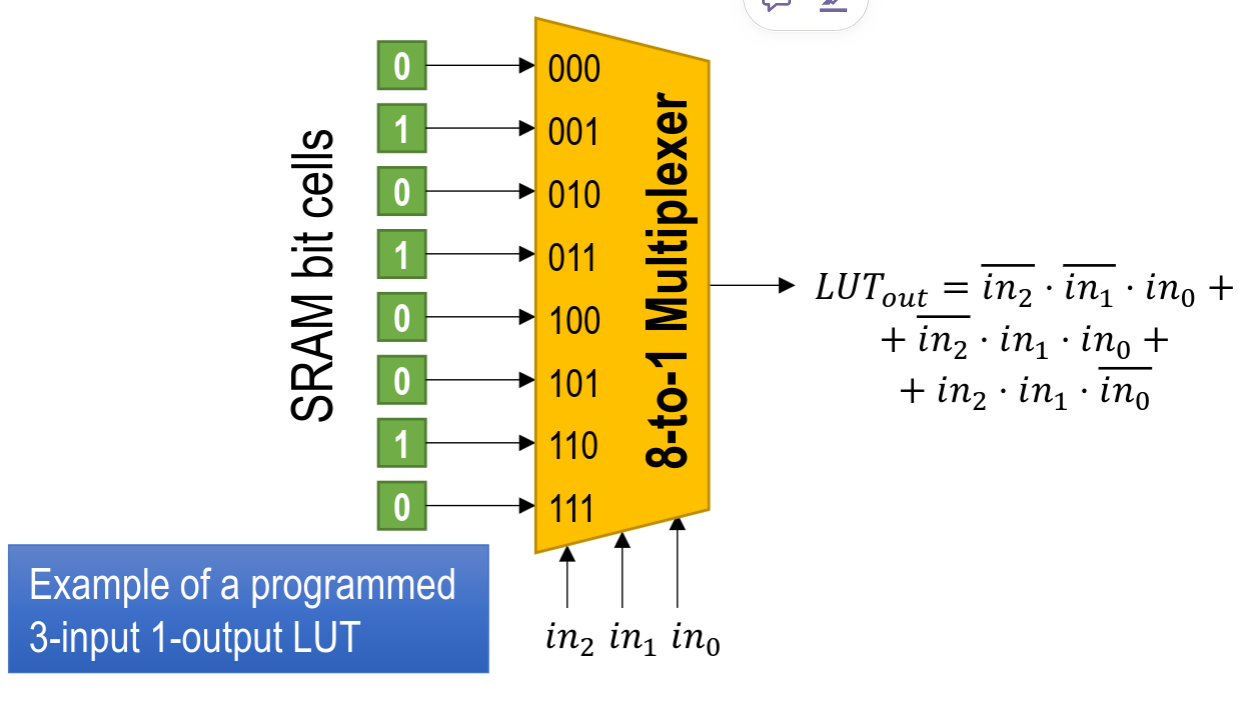
\includegraphics[scale=0.25]{../figures/fpga_lut.png}
\end{center}

\subsubsection{Interconnections}

Interconnections in FPGAs are usually implemented via \textbf{switch matrices}, usually made up of 6 pass transistors.

\begin{center}
	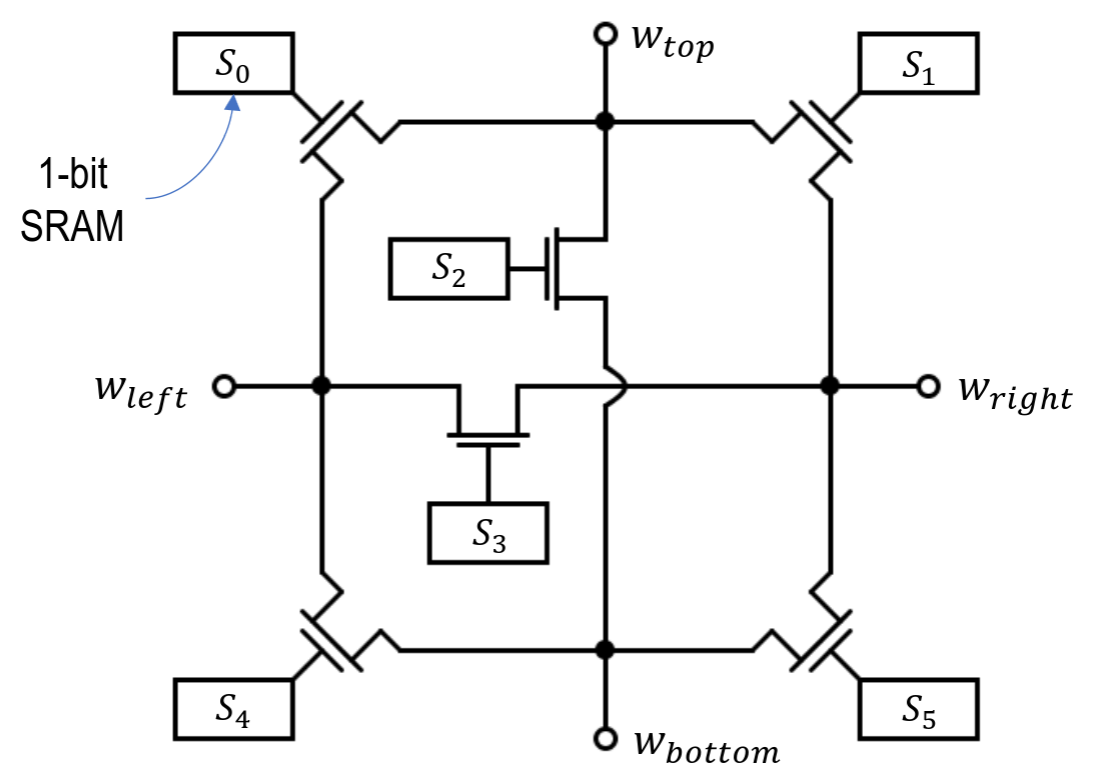
\includegraphics[scale=0.22]{../figures/swima.png}
\end{center}

It is pretty clear how, by changing the contents of the control SRAM we can change the thresholds of the pass transistors and thus the pairs of nodes across $w_\text{top}$, $w_\text{right}$, $w_\text{bottom}$ and $w_\text{left}$, creating any kind of interconnection.

\begin{center}
	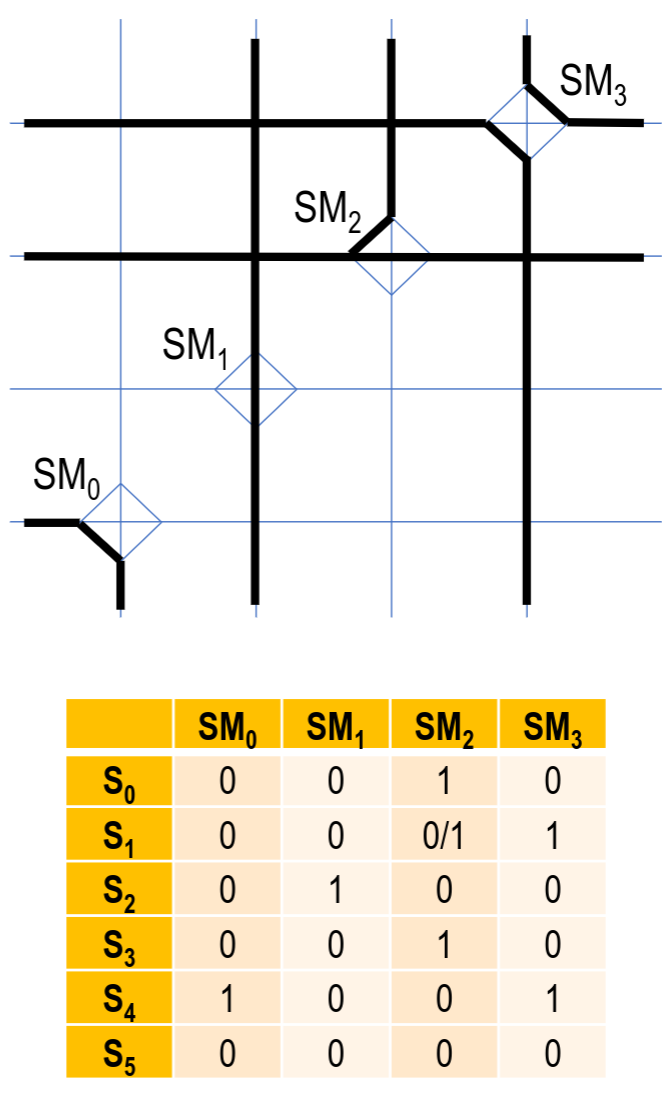
\includegraphics[scale=0.22]{../figures/swima_conn.png}
\end{center}

A switch matrix divides wires into independent segments.
Segments are connected by properly activating transistors in the switch matriix.
If not connected, adjacent segments may belong to different interconnections, with no conflicts because inactive transistors separate them.

Because a switch matrix introduces delays and increases the area, we tend to limit the number of switch matrices to improve performance and decrease costs.
On the other hand a switch matrix increases flexibility, and more switch matrices make routing easier.

\subsubsection{I/O blocks}

FPGAs also feature \textbf{I/O blocks} such as the ones saw for CPLDs in 12.1.
Because FPGAs are usually more complex, though, the I/O blocks are usually more complex too.
In this they have:
\begin{itemize}
\item Output buffer with Enable signal;
\item Combinational or sequential inputs and outputs;
\item Optional Pull-Up, Clamp and Bus Hold circuits, configurable by controlling the selection signals of multiplexers
\end{itemize}

\begin{center}
	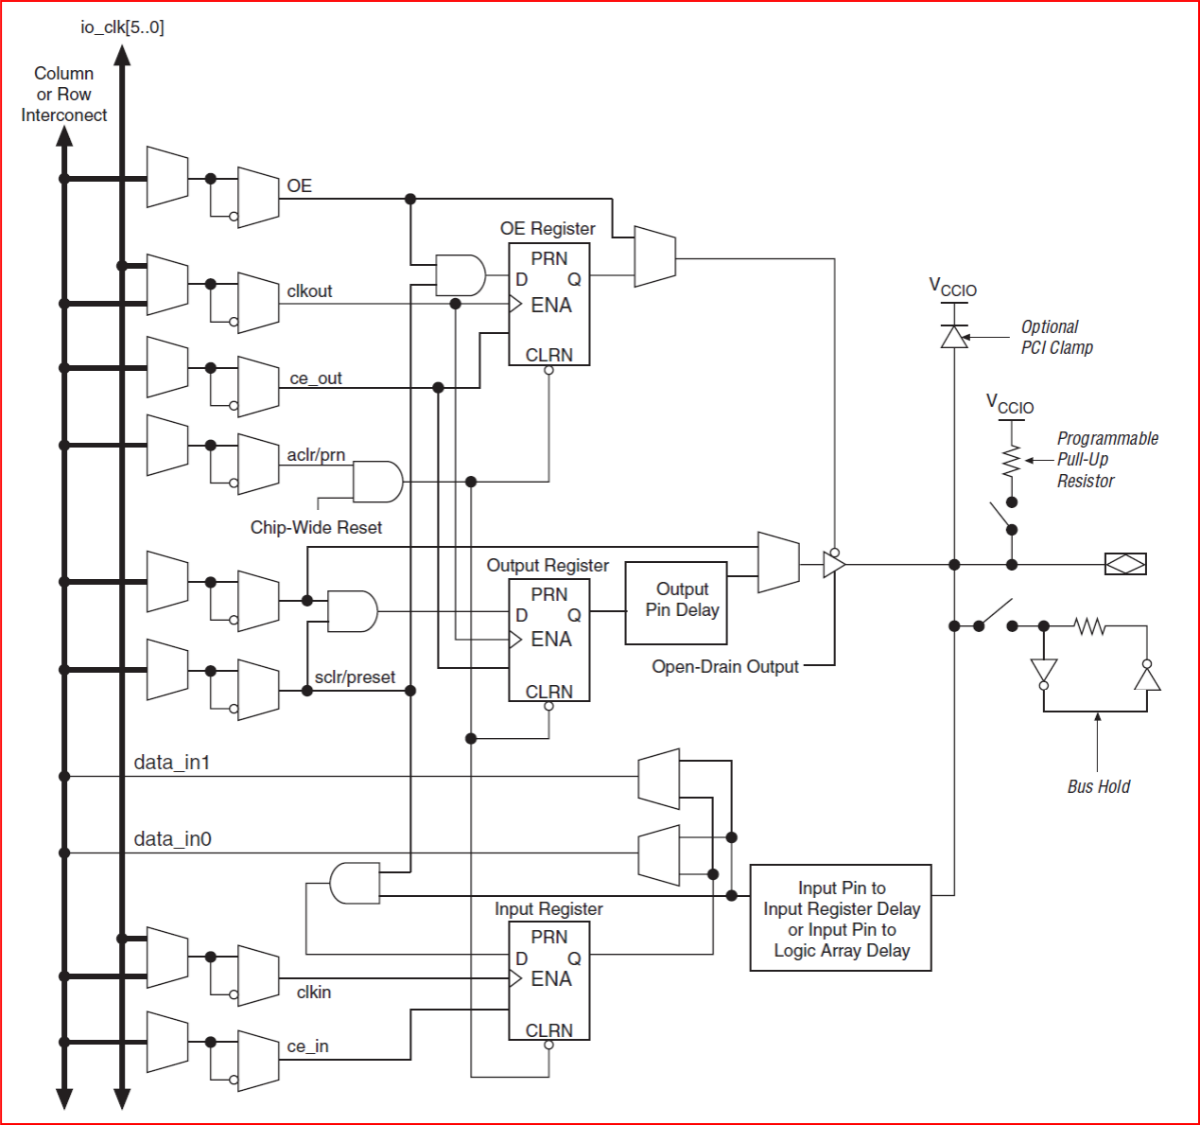
\includegraphics[scale=0.22]{../figures/ioblock_fpga.png}
\end{center}

\subsubsection{Additional FPGA blocks}

FPGAs, being more complex and versatile than other logic devices, usually feature additional blocks such as:
\begin{itemize}
	\item \textbf{Memories} and \textbf{FIFO} (\textit{First-In, First-Out}) queues.
		These are usually SRAMs, but not control SRAM cells like we saw before: actual SRAM topologies in the order of kilobytes, with address decoders and bit multiplexers.
		Sometimes interfaces for external dynamic memories are available.

	\item  \textbf{Carry chains} between different CLBs or LEs: these allow implementing efficient adders;
	\item Embedded hardware \textbf{multipliers} or \textbf{DSP} (\textit{Digital Signal Processing}) blocks;
	\item Clock management circuitry;
	\item High speed \textbf{I/O};
	\item Even \textbf{processor cores}.
\end{itemize}

\subsubsection{FPGA performance}

Let's do a few performance and design considerations.
First off, the kind of technology used to program the FPGA is slighlty varied:
\begin{itemize}
	\item \textbf{SRAM} is dominant, used for LUTs, but also to control MUXes or pass transistors. Controlling standard CMOS technology, it can be reprogrammed on the fly, which makes for a standard technology which allows to easily embed other blocks (which is the reason FPGAs are usually at the cutting-edge of a given technology).
The main con is the large size, power consumption, and the fact that SRAM is not permanent;
\item \textbf{Fuse and Antifuse} is sometimes used as its small and permanent, but it cannot be reprogrammed nor tested;
\item \textbf{EEPROM} or \textbf{Flash} can be reprogrammed, but don't represent a standard proces.
\end{itemize}

We can then compare to other PLD technologies, namely \textbf{CPLD}s.

FPGAs are configured at a finer level than CPLDs, which have few large configurable blocks, while FPGAs have many small configurable blocks. FPGAs are volatile, typically implemented using SRAM technology, and must be reprogrammed at every power-up, whereas CPLDs are non-volatile, typically using EEPROM technology. FPGAs use standard technology, making it easier to include additional resources. They are more expensive, but cheaper per gate, and usually much larger. CPLDs are more predictable, while FPGA delays can vary significantly with the implementation.

\subsection{FPGA design flow}

We know come to the \textbf{design} part of using FPGAs.

\begin{center}
	\includegraphics[scale=0.22]{../figures/fgpa_design.png}
\end{center}

This is easier than wrangling LUTs manually, as it usually involves:
\begin{enumerate}
	\item \textbf{Specification} and \textbf{Design Entry}, through specialized hardware description language such as VHDL, Verilog, SystemC, Chisel, HLS.
	\item \textbf{Behavioral Simulation}, that is the execution of the specification, with no timing information, needed to verify the algorithm and quickly explore the design space;
	\item \textbf{Initial Synthesis}, which generates synthesizable boolean expressions independent of the target implementation;
	\item \textbf{Functional Simulation}: similar to Behavioral Simulation, also known as \textbf{RTL} (\textit{Register Transfer Level}) simulation. This still has no timing information;
	\item \textbf{Logic Synthesis}. This is the hard part. It involves echnology independent optimizations, technology mapping and Place \& Route. At this point we need a device model to be known, provided by the manufacturer, and we need the pin assignments.
	Logic synth. is driven by timing constraints, as we want to look for best implementation on a given technology. As we said, it's a very complex problem, solved via simulated annealing, genetic algorithms, ecc... which may get different results at any run;
\item \textbf{Timing analysis} and \textbf{Timing Simulation}: we can finally compare the circuit with timing constraints, also known as gate level simulation. This is far slower than other simulation kinds;
\item \textbf{Assembler}: generates the Bit Stream for the target device, and as such all SRAM configuration bits;
\item \textbf{Programmer} writes the Bit Stream on the actual device through its JTAG Interface. The SRAM acts like a very long shift register, which is serially programmed, to reduce pin counts (and allow JTAG chaining, more on the good ol'wikipediaz).
\end{enumerate}

\end{document}
